\section{Cơ sở lý thuyết}
\subsection{Hệ thống Định vị Toàn cầu GPS}
\subsubsection{GPS là gì}
GPS là hệ thống định vị toàn cầu dựa trên mạng lưới các vệ tinh nhân tạo quay quanh Trái Đất. Hệ thống này được thiết kế, xây dựng và vận hành bởi Bộ Quốc phòng Hoa Kỳ, ban đầu phục vụ mục đích quân sự, sau đó mở rộng cho dân sự từ thập niên 1980.

\subsubsection{Cấu trúc hệ thống}
GPS gồm ba thành phần chính:
\begin{itemize}
    \item Phần không gian (Space Segment): gồm 30 vệ tinh (27 vệ tinh hoạt động và 3 vệ tinh dự phòng) nằm trên các quỹ đạo xoay quanh Trái Đất. Chúng cách mặt đất 20.200 km, bán kính quỹ đạo 26.600 km. Chúng chuyển động ổn định và quay hai vòng quỹ đạo trong khoảng thời gian gần 24 giờ với vận tốc 7 nghìn dặm một giờ. Các vệ tinh trên quỹ đạo được bố trí sao cho các máy thu GPS trên mặt đất có thể nhìn thấy tối thiểu 4 vệ tinh vào bất kỳ thời điểm nào.
    \item Phần điều khiển (Control Segment): kiểm soát vệ tinh đi đúng hướng theo quỹ đạo và thông tin thời gian chính xác. Có 5 trạm kiểm soát đặt rải rác trên Trái Đất. Bốn trạm kiểm soát hoạt động một cách tự động, và một trạm kiểm soát là trung tâm. Bốn trạm này nhận tín hiệu liên tục từ những vệ tinh và gửi các thông tin này đến trạm kiểm soát trung tâm. Tại trạm kiểm soát trung tâm, nó sẽ sửa lại dữ liệu cho đúng và kết hợp với hai an-ten khác để gửi lại thông tin cho các vệ tinh. Ngoài ra, còn một trạm kiểm soát trung tâm dự phòng và sáu trạm quan sát chuyên biệt.
    \item Phần người dùng (User Segment): các thiết bị thu GPS (điện thoại, ô tô, tàu thuyền, máy bay…).
\end{itemize}

\subsubsection{Nguyên lý hoạt động}
\begin{itemize}
    \item Mỗi vệ tinh GPS phát tín hiệu chứa thời gian phát và vị trí chính xác $(x_i,y_i,z_i)$ của vệ tinh tại thời điểm đó. 
    \item Thiết bị thu GPS nhận tín hiệu và so sánh thời gian phát với thời gian nhận → tính được khoảng cách đến vệ tinh $R_i$.
    \item Để xác định vị trí trong không gian 3D, cần ít nhất 4 vệ tinh:
    \begin{itemize}
        \item 3 vệ tinh để tính vĩ độ, kinh độ, độ cao.
        \item 1 vệ tinh bổ sung để hiệu chỉnh sai số đồng hồ trong thiết bị thu.
    \end{itemize}
\item Giải hệ phương trình 4 ẩn sau, ta được (X,Y,Z) là tọa độ thiết bị thu. Với $(x_i,y_i,z_i)$ là tọa độ các vệ tinh tương ứng, $R_i$ là khoảng cách tự vệ tinh tới thiết bị nhận, c là vận tốc ánh sáng trong chân không, $t_i$ là thời gian phản hồi từ vệ tinh đến thiết bị nhận, $\Delta t$ là sai số giữa vệ tinh và thiết bị nhận.
    \begin{align}
 R_{1} = \sqrt{(X - x_{1})^{2} + (Y - y_{1})^{2} + (Z - z_{1})^{2}} = c \bigl( t_{1} - t_{0} \pm \Delta t \bigr) \
\\
R_{2} = \sqrt{(X - x_{2})^{2} + (Y - y_{2})^{2} + (Z - z_{2})^{2}} 
      = c \bigl( t_{2} - t_{0} \pm \Delta t \bigr) \
\\
R_{3} = \sqrt{(X - x_{3})^{2} + (Y - y_{3})^{2} + (Z - z_{3})^{2}} 
      = c \bigl( t_{3} - t_{0} \pm \Delta t \bigr) \
\\
R_{4} = \sqrt{(X - x_{4})^{2} + (Y - y_{4})^{2} + (Z - z_{4})^{2}} 
      = c \bigl( t_{4} - t_{0} \pm \Delta t \bigr)
    \end{align}

    

\end{itemize}
\subsubsection{Dữ liệu GPS}
Các thiết bị GPS hiện đại xuất ra dữ liệu định vị toàn cầu dựa vào quan sát tối thiểu 4 vệ tinh để xác định vị trí 3D (lat, lon, alt) với độ trễ thấp và độ chính xác phụ thuộc số lượng vệ tinh hữu ích, điều kiện môi trường, model thiết bị thu.

\begin{itemize}
    \item Định dạng truyền dẫn tiêu chuẩn: NMEA-0183, RINEX, RTCM... Trong hệ nhúng/robotics phổ biến nhất là dòng NMEA (GGA, RMC...) cung cấp nhanh các tham số tọa độ, chất lượng tín hiệu, số vệ tinh, độ chính xác đo lường, vận tốc v.v...
    \item Mã hóa thông điệp: giá trị vĩ độ, kinh độ (thập phân, DMS), độ cao (so với mực nước biển), thông số chất lượng (HDOP, VDOP), và tín hiệu thời gian chuẩn UTC.
\end{itemize}
\textbf{Các lỗi phổ biến khi lấy dữ liệu GPS}: che chắn/vật cản, nhiễu đa đường, nhiễu sóng, sai số đồng bộ thời gian, sai số khí quyển (điện ly, đối lưu), bị spoofing/jamming tấn công.

\subsection{Tam giác cầu}
\subsubsection{Định nghĩa và tính chất}
Tam giác cầu là hình được tạo thành bởi ba cung tròn lớn cắt nhau trên mặt cầu. Mỗi cạnh là một cung tròn lớn, còn các góc là giao của hai cung đó. Độ dài của cạnh không phải đo bằng độ dài (đơn vị mét) mà đo bằng góc ở tâm (tính bằng độ hoặc radian), bằng cung tròn nối hai điểm trên mặt cầu chia cho bán kính. Xuất hiện trong nhiều lĩnh vực thực tế: hàng hải, hàng không, thiên văn, đo đạc bản đồ, định hướng vệ tinh, quân sự...
\subsubsection{Mối Liên Hệ Lượng Giác Cầu Và Vector Định Hướng 3D}
Phép toán hình học giữa các điểm trên cầu có thể mô tả bằng tích vô hướng, tích có hướng, chuyển đổi tọa độ từ kinh vĩ độ sang vector 3D (n-vector):
\begin{itemize}
    \item Với điểm trên cầu có \textbf{vĩ độ $\phi$, kinh độ $\lambda$}:
    \begin{center}
        $x = Rcos\phi cos\lambda$ \\
        $y = Rcos\phi sin\lambda$ \\
        $z = Rsin\phi$ \\
    \end{center}
\item Đây là nền tảng chuyển đổi dữ liệu địa lý sang không gian vector 3D, phục vụ cho các thuật toán dẫn đường, định hướng, hoặc mô phỏng quỹ đạo trên cầu. Từ vector 3D suy trở lại kinh vĩ độ.

\end{itemize}

\subsection{Phép Chiếu Bản Đồ}
\subsubsection{Khái niệm}
Phép chiếu bản đồ là phép toán học chuyển bề mặt cong 3D của Trái đất (hình cầu, ellipsoid) lên mặt phẳng bản đồ 2D. Không một phép chiếu nào bảo toàn toàn bộ hình dạng, diện tích, góc và khoảng cách. Các phép chiếu được tạo ra để tối ưu hóa một hoặc một vài thuộc tính tùy mục đích sử dụng.
\subsubsection{Các Phép Chiếu Bản Đồ Phổ Biến}
\begin{itemize}
    \item Phép Chiếu Hình Trụ (Cylindrical Projection): Chiếu điểm cầu lên hình trụ "bao" quanh quả cầu, sau đó trải phẳng.
    \begin{itemize}
        \item Ưu điểm: Giữ vững góc tại xích đạo, thích hợp cho khu vực quanh xích đạo. Đường kinh tuyến và vĩ tuyến đều là đường thẳng song song, vuông góc nhau, dễ biểu diễn, thuận tiện cho đo đạc các vị trí gần đường tiếp xúc.
        \item Nhược điểm: Biến dạng tăng dần về phía cực, diện tích các khu vực gần cực bị phóng đại mạnh. Không áp dụng tốt với lãnh thổ trải dài Bắc - Nam hoặc khu vực cực.
    \end{itemize}
    \item Phép Chiếu Mercator (Mercator Projection): Là hình trụ đứng đồng góc, công thức ($\lambda$ là kinh độ, $\phi$ là vĩ độ, $\lambda _0$ là kinh tuyến chuẩn: 
    \begin{center}
        $x = R(\lambda - \lambda _0)$
        $y = R.ln(tan(\pi/4 + \phi/2))$
    \end{center}
    \begin{itemize}
        \item Ưu điểm: Bảo toàn góc (hữu ích cho định hướng, hướng đi hàng hải, tuyến đường thẳng trên bản đồ là tuyến đường không đổi hướng la bàn). Dễ dàng chuyển đổi số liệu, tích hợp vào bản đồ WebGIS toàn cầu (Google Maps, OSM, Bing Maps đều dùng biến thể Mercator).
        \item Nhược điểm: Biến dạng diện tích tăng rất mạnh về phía cực (ví dụ Greenland gần như lớn bằng châu Phi trên bản đồ Mercator); chỉ phù hợp thực tế cho vùng gần xích đạo.
    \end{itemize}
    \item Phép Chiếu UTM (Universal Transverse Mercator)
    \begin{itemize}
        \item Là phép chiếu hình trụ ngang đồng góc, chia toàn cầu thành 60 múi, mỗi múi rộng 6 độ kinh độ (với số hiệu từ 1-60, bắt đầu từ 180° Tây).
        \item Sử dụng trục hình trụ cắt cầu tại hai đường cong gần múi trung tâm (giảm biến dạng, phân bổ đều sai số).
        \item Kinh tuyến giữa có hệ số biến dạng k < 1 (thường k = 0.9996).
        \item Biến dạng nhỏ, đều; phù hợp cho bản đồ tỷ lệ lớn, khu vực có diện tích lớn, lãnh thổ trải dài đông-tây/north-south. Là tiêu chuẩn toàn cầu trong trắc địa, quân sự, GPS, QGIS, hệ thống VN2000.
        \item Nhược điểm: Đòi hỏi thay đổi múi chiếu khi vượt biệt khu vực rộng, cần căn chỉnh số hiệu múi cho phù hợp từng khu vực.
    \end{itemize}
\end{itemize}

\subsection{Hệ Tọa Độ Không Gian}
\subsubsection{Hệ tọa độ trắc địa Geodetic (Kinh độ, Vĩ độ, Độ cao)}
Hệ tọa độ Geodetic (toạ độ trắc địa) mô tả vị trí một điểm trên bề mặt hoặc gần bề mặt Trái Đất bằng 3 tham số:
\begin{itemize}
    \item Vĩ độ: Góc lệch giữa mặt phẳng xích đạo và phương đi qua tâm trái đất đến điểm cần xác định. Giá trị từ -90° (cực Nam) đến +90° (cực Bắc).
    \item Kinh độ: Góc giữa kinh tuyến đi qua điểm cần xác định và kinh tuyến gốc tại Greenwich, chạy từ -180° tới 180°.
    \item Độ cao: Khoảng cách vuông góc từ điểm cần xác định tới mặt elip tham chiếu (ellipsoid), đơn vị thường là mét.
\end{itemize}
\subsubsection{Hệ tọa độ địa tâm địa cố ECEF (Earth-Centered, Earth-Fixed)}
Hệ tọa độ ECEF là hệ tọa độ Đề-các (vuông góc) ba chiều, có:
\begin{itemize}
    \item Gốc tọa độ: Tâm Trái Đất.
    \item Trục X: Đi qua giao điểm giữa mặt phẳng xích đạo và kinh tuyến gốc Greenwich (vĩ độ 0°, kinh độ 0°).
    \item Trục Y: Nằm trong mặt phẳng xích đạo, cách trục X 90° về phía đông (vĩ độ 0°, kinh độ 90°).
    \item Trục Z: Trùng với trục quay của Trái Đất, hướng về phía cực Bắc (vĩ độ 90°).
\end{itemize}
\textbf{Đặc điểm}: ECEF là hệ tọa độ tuyệt đối, xoay đồng bộ với Trái Đất. Đơn vị là mét. Các điểm có tọa độ (X, Y, Z) trong ECEF có thể là điểm trên mặt đất, trong khí quyển, quỹ đạo vệ tinh hoặc ngoài không gian lân cận Trái Đất1.
\subsubsection{Hệ tọa độ ENU (East-North-Up)}
ENU là hệ tọa độ địa phương (Local Tangent Plane Coordinates), với:
\begin{itemize}
    \item Gốc tọa độ đặt tại một điểm tham chiếu (người quan sát).
    \item Trục X - East: Hướng về phía Đông địa phương.
    \item Trục Y - North: Hướng về phía Bắc địa phương.
    \item Trục Z - Up: Hướng thẳng đứng lên trên (vuông góc với mặt ellipsoid tại điểm gốc).
\end{itemize}
Hệ ENU thuận tay phải, rất phù hợp cho các thuật toán điều hướng, robot, dẫn đường UAV, phân tích radar hoặc quy hoạch đô thị, khi các tính toán chỉ cần tập trung vào phạm vi một vùng nhỏ xung quanh người quan sát.
\subsubsection{Hệ tọa độ NED (North-East-Down)}
NED là hệ tọa độ định hướng cục bộ nổi bật trong ngành hàng không, tàu biển, mô phỏng quán tính:
\begin{itemize}
    \item Trục X - North: Hướng về phía Bắc địa phương.
    \item Trục Y - East: Hướng về phía Đông địa phương.
    \item Trục Z - Down: Hướng thẳng đứng xuống dưới (vuông góc với mặt ellipsoid, phía tâm Trái đất).
\end{itemize}
Hai hệ ENU và NED chỉ khác nhau thứ tự trục: NED có Z hướng xuống (“down” dương), phù hợp với một số ứng dụng động lực học tàu bay, tàu biển - các vật thể chủ yếu di chuyển/quan sát phía dưới máy bay.
\newpage
\subsubsection{Hệ quy chiếu ellipsoid chuẩn WGS-84}
Để đảm bảo các phép chuyển đổi thông suốt và nhất quán trên toàn cầu, WGS-84 (World Geodetic System 1984) là ellipsoid tham chiếu thống nhất cho GPS - với các tham số: \\
\begin{table}[h!]
\centering
\begin{tabular}{|l|c|c|c|}
\hline
\textbf{Tham số}     & \textbf{Ký hiệu} & \textbf{Giá trị}        & \textbf{Đơn vị} \\ \hline
Bán trục lớn         & $a$              & 6,378,137.0             & m              \\ \hline
Độ dẹt               & $f$              & $1/298.257223563$       & -              \\ \hline
Độ lệch tâm          & $e$              & 0.0818191908426         & -              \\ \hline
$e^2$                & $e^2$            & 0.0066943799901377997        & -              \\ \hline
Bán trục nhỏ         & $b$              & 6,356,752.3142          & m              \\ \hline
\end{tabular}
\caption{Các tham số elipsoid WGS-84}
\end{table}
\\
WGS-84 là mặt ellipsoid sát nhất mô phỏng hình dạng Trái Đất, được duy trì thường xuyên để thích hợp với di động kiến tạo mảng, mực nước biển và biến động trọng lực toàn cầu.


\subsection{Chuyển đổi giữa các hệ tọa độ}
\subsubsection{Chuyển đổi Geodetic $(\varphi, \lambda, h)$ sang ECEF $(X, Y, Z)$}
\begin{itemize}
    \item $\varphi$: vĩ độ tính bằng radian
    \item $\lambda$ kinh độ tính bằng radian
    \item h: cao độ so với ellipsoid
    \item a: bán trục lớn của ellipsoid
    \item e: độ lệch tâm của ellipsoid
    \begin{enumerate}
        \item Tính N (bán kính cong đơn vị kinh tuyến chính):
        \begin{center}
            $N = \frac{a}{\sqrt{1 - e^2sin2\varphi}}$
        \end{center}
        \item Tọa độ ECEF:
        \begin{center}
$$
\begin{aligned}
X &= (N + h) \cdot \cos\varphi \cdot \cos\lambda \\
Y &= (N + h) \cdot \cos\varphi \cdot \sin\lambda \\
Z &= \left[N \cdot (1 - e^2) + h\right] \cdot \sin\varphi
\end{aligned}
$$


        \end{center}
    \end{enumerate}
\end{itemize}

\subsubsection{Chuyển đổi ECEF $\leftrightarrow$ ENU}
\subsubsubsection{Từ ECEF sang ENU}
\begin{itemize}
  \item Giả sử điểm gốc \textit{local origin} có tọa độ địa lý $(\phi_0, \lambda_0, h_0)$ — tính được tọa độ ECEF: $(X_0, Y_0, Z_0)$.
  \item Tính vector sai khác:
  

\[
  \Delta = 
  \begin{bmatrix}
  dX \\
  dY \\
  dZ
  \end{bmatrix}
  =
  \begin{bmatrix}
  X - X_0 \\
  Y - Y_0 \\
  Z - Z_0
  \end{bmatrix}
  \]


  \item Xoay $\Delta$ bằng ma trận quay $R$ để đưa về hệ trục ENU:
  

\[
  \begin{bmatrix}
  E \\
  N \\
  U
  \end{bmatrix}
  =
  \begin{bmatrix}
  -\sin\lambda_0 & \cos\lambda_0 & 0 \\
  -\sin\phi_0\cos\lambda_0 & -\sin\phi_0\sin\lambda_0 & \cos\phi_0 \\
  \cos\phi_0\cos\lambda_0 & \cos\phi_0\sin\lambda_0 & \sin\phi_0
  \end{bmatrix}
  \begin{bmatrix}
  dX \\
  dY \\
  dZ
  \end{bmatrix}
  \]


  \item Kết quả là tọa độ $(E, N, U)$ trong hệ ENU tại gốc $(\phi_0, \lambda_0, h_0)$.
\end{itemize}

\subsubsubsection{Từ ENU sang ECEF}
Đảo ngược phép quay và chuyển vị trí, tức là áp dụng ma trận chuyển đổi nghịch đảo (hoặc chuyển vị) để đưa tọa độ ENU về lại hệ ECEF.


\subsubsection{Chuyển đổi ECEF $\leftrightarrow$ NED}

Hai hệ ENU và NED chỉ khác thứ tự trục và một số dấu:


\[
[N, E, D] = [E, N, U] \quad \text{với } D = -U
\]



Ma trận quay cho NED về ECEF cũng có dạng gần giống ENU, chỉ đảo trục dọc trục đứng.


\subsection{Góc Azimuth và Elevation}
\subsubsection{Azimuth (Góc phương vị)}
Azimuth là góc nằm ngang trên mặt phẳng XY, xác định hướng nhìn hay hướng ngắm mục tiêu so với hướng chuẩn (thường là hướng Bắc địa lý). Trong các hệ ENU/NED, azimuth được quy ước như sau:
\begin{itemize}
    \item Azimuth = 0° tương ứng hướng Bắc.
    \item Được đo theo chiều kim đồng hồ từ Bắc - tức là hướng Đông là 90°, Nam là 180°, Tây là 270°.
\end{itemize}
\subsubsection{Elevation (Góc nâng)}
Elevation là góc giữa vector quan sát với mặt phẳng ngang (XY) tại vị trí người quan sát:
\begin{itemize}
    \item Góc elevation = 0°: hướng song song mặt đất (horizon).
    \item Góc elevation > 0°: hướng lên trên đường chân trời.
    \item Góc elevation < 0°: hướng xuống dưới mặt phẳng chân trời.
\end{itemize}
\textbf{Ký hiệu: }elevation thường dùng đơn vị độ (°), hoặc radian.

\subsubsection{Chuyển Azimuth/Elevation Thành Vector Định Hướng Trong ENU/NED}
\subsubsubsection{Vector định hướng trong ENU}
Giả sử bạn nhận được các giá trị azimuth (A) và elevation (E) ở độ, vector hướng trong hệ ENU sẽ là:
$$
\begin{aligned}
x_{ENU} &= cos(E).sin(A) \\
y_{ENU} &= cos(E).cos(A) \\
z_{ENU} &= sin(E) \\
\end{aligned}
$$
\textbf{Quy ước quan trọng: }
\begin{itemize}
    \item Azimuth A: 0° hướng Bắc (Y+), 90° hướng Đông (X+).
    \item Elevation E: 0° nằm ngang, +90° thẳng đứng lên (Z+).
\end{itemize}

\subsubsubsection{Vector định hướng trong NED}
Khác biệt lớn nhất ở hệ NED là trục Z hướng xuống:

$$
\begin{aligned}
x_{NED} &= cos(E).cos(A) \\
y_{NED} &= cos(E).sin(A) \\
z_{NED} &= - sin(E) \\
\end{aligned}
$$
\textbf{Ghi chú quy ước:}
\begin{itemize}
    \item Azimuth vẫn tính như ENU, nhưng trục đặt lại.
    \item Độ dương/âm của thành phần z thay đổi để đảm bảo Z hướng xuống.
\end{itemize}

\subsection{Xác định điểm mục tiêu từ vector định hướng và khoảng cách đo bằng laser}
\begin{itemize}
    \item Lấy vị trí người quan sát làm gốc hệ ENU.
    \begin{itemize}
        \item Trong không gian 3D, để đơn giản hóa các phép tính hướng và vị trí, thường quy ước đặt gốc hệ ENU trùng với vị trí người quan sát trên mặt đất. Trục Ox (East) hướng về phía Đông, Oy (North) hướng về phía Bắc, Oz (Up) vuông góc mặt đất và hướng lên trời.
        \item Khi gốc tọa độ được cố định tại người quan sát, bất kỳ điểm nào trong không gian gần gốc (phạm vi vài km) sẽ được biểu diễn nhờ ba giá trị ENU (E: Đông, N: Bắc, U: Cao). Điều này giúp phép cộng, trừ vector và chuyển đổi hệ dễ thực hiện hơn.
        \item Ví dụ: Nếu một trạm đo đặt tại (lat0, lon0, h0), là gốc ENU, điểm mục tiêu sẽ tính toán tương đối với gốc này.
    \end{itemize}
    \item Tính vector định hướng 3D từ azimuth, elevation (như phần 2.6.3)
    \item Xác định tọa độ mục tiêu trong ENU bằng phép cộng vector
    \begin{itemize}
        \item Sau khi đã có vector định hướng 3D đơn vị V, tọa độ mục tiêu trong ENU sẽ được tính bằng phép cộng vị trí người quan sát với khoảng cách đo được nhân vector định hướng:
$$
\begin{aligned}
P_{target\_ENU} &= P_{oberserver\_ENU} + D.V
\end{aligned}
$$
\textbf{Trong đó:}
    \item $P_{target\_ENU}$ = (0,0,0) do lấy người quan sát là gốc
    \item D là khoảng cách đo bằng laser (đơn vị mét)
    \item V là vectơ định hướng 3D đơn vị đã tính
    \end{itemize}
    \item Chuyển ENU sang ECEF
    Công thức ma trận chuyển đổi: $P_{ECEF} = R_{ENU \rightarrow ECEF} . P_{ENU} + Observer_{ECEF}$ \\
    Trong đó: 
    

\[
R = \begin{pmatrix}
-\sin\lambda & -\sin\phi\cos\lambda & \cos\phi\cos\lambda \\
\cos\lambda & -\sin\phi\sin\lambda & \cos\phi\sin\lambda \\
0 & \cos\phi & \sin\phi
\end{pmatrix}
\]

\begin{itemize}
    \item $\lambda$ là kinh độ, $\phi$ là vĩ độ, $Observer_{ECEF}$ được tính theo phần 2.5.1
\end{itemize}
    \item Chuyển ECEF sang địa lý (kinh vĩ độ, cao độ)
    Từ điểm ECEF (X, Y, Z), chuyển về hệ tọa độ địa lý dùng công thức chuẩn WGS84($\lambda$,$\phi$,$h$):
    

\[
\lambda = \arctan2(Y, X)
\]

\[
p = \sqrt{X^2 + Y^2}
\]

\[
\phi = \arctan \!\left( 
   \frac{Z}{p} \cdot 
   \left( 1 - e^2 \cdot \frac{a}{\sqrt{p^2 + (1 - e^2)Z^2}} \right)^{-1} 
\right)
\]

\[
h = \frac{p}{\cos\phi} - N(\phi)
\]

\[
N(\phi) = \frac{a}{\sqrt{1 - e^2 \sin^2\phi}}
\]
    \begin{itemize}
        \item Với các thông số xem lại trong bảng 1
    \end{itemize}

\end{itemize}
\newpage
\section{Xử lý dữ liệu cảm biến GPS, IMU và Laser}
\subsection{Giới thiệu và đặc tính từng loại cảm biến}
\subsubsection{IMU (Inertial Measurement Unit)}
IMU là tổ hợp nhiều cảm biến: accelerometer (gia tốc kế), gyroscope (con quay hồi chuyển), magnetometer (la bàn số) cung cấp thông tin về gia tốc tuyến tính, vận tốc góc, phương hướng và trường từ trường của môi trường.
\begin{itemize}
    \item Accelerometer: đo gia tốc (bao gồm cả trọng lực), dùng xác định phương trọng lực, đo rung động.
    \item Gyroscope: đo vận tốc quay, giúp xác định thay đổi hướng, tính toán góc nghiêng, phục vụ tính toán quán tính.
    \item Magnetometer: đo trường từ, dùng định hướng Bắc-Tây-Nam, hỗ trợ hiệu chuẩn phương vị.
    \item \textbf{Thông số cơ bản:}
    \begin{itemize}
      \item Dải đo \textbf{accelerometer}: $\pm 2g \ldots \pm 16g$, 
            noise density đến $0.01$ -- $0.02 \,m/s^2/\sqrt{Hz}$.
            
      \item Dải đo \textbf{gyroscope}: lên tới $\pm 2000^{\circ}/\text{s}$, noise density tầm $0.1$--$0.15^{\circ}/\text{s}/\sqrt{\text{Hz}}$; 
            bias thường là vài $^{\circ}/\text{h}$ (tốt) đến vài trăm $^{\circ}/\text{h}$ (rẻ).
            
      \item \textbf{Magnetometer}: độ nhạy tới $\sim 1\,\mu\text{T}$ (microtesla), 
            noise $< 0.5\,\mu\text{T}/\sqrt{Hz}$.
    \end{itemize}
\end{itemize}
IMU hiện diện rộng rãi trong robot di động, máy bay không người lái UAV, xe hơi tự hành, máy đo chuyên dụng phục vụ đo đạc bản đồ, dò tìm dị thường địa vật lý.

\subsubsection{Laser Rangefinder}
Laser Rangefinder là thiết bị đo khoảng cách chính xác dựa trên nguyên lý lan truyền của xung laser, hoạt động dựa trên time-of-flight, phase-shift hoặc triangulation.
\begin{itemize}
    \item \textbf{Nguyên lý cơ bản:}
    \begin{itemize}
        \item Time-of-flight: bắn xung laser → đo thời gian tới-lui → tính khoảng cách.
        \item Phase-shift: đo độ lệch pha giữa sóng phát và sóng phản xạ, cho độ chính xác cao ở tầm gần và trung bình.
        \item Triangulation: dùng định vị hình học điểm chiếu, chủ yếu cho đo dịch chuyển nhỏ, độ phân giải cao.
    \end{itemize}
    \item \textbf{Độ chính xác:} Tùy cấu hình, có thể xuống tới 0.1mm (triangulation), cấp mm-cm (time-of-flight), sub-mm (phase-shift). Khoảng đo tới vài chục mét (nhỏ, dùng trong công nghiệp), tới vài km (quân sự).
    \item \textbf{Yếu tố ảnh hưởng:} Độ ẩm, bụi, mưa/động học khí quyển, mục tiêu hoặc vật cản, phân kỳ tia, hiệu ứng môi trường làm suy hao tín hiệu, độ phản xạ bề mặt mục tiêu.
\end{itemize}

\subsection{Các lỗi cảm biến và ảnh hưởng đến hệ thống định vị}
\subsubsection{Lỗi GPS} 
\begin{table}[h!]
\centering
\begin{tabular}{|l|p{7cm}|c|}
\hline
\textbf{Loại lỗi} & \textbf{Mô tả} & \textbf{Độ lớn (m)} \\
\hline
Ionospheric delay & Sai số do tín hiệu đi qua tầng ion, phụ thuộc tần số, khắc phục L1/L2 & $\pm 5$--$50$ \\
\hline
Tropospheric delay & Sai số do hơi ẩm, áp suất khí quyển & $\pm 0.5$--$30$ \\
\hline
Multipath distortion & Phản xạ đa đường (địa hình, mặt nước, nhà cửa) & $\pm 1$--$150$ \\
\hline
Ephemeris errors & Quỹ đạo vệ tinh bị lỗi thời gian, sai vị trí vệ tinh & $\pm 2$--$5$ \\
\hline
Satellite clock drift & Trôi đồng hồ nguyên tử trên vệ tinh & $\pm 0$--$1.5$ \\
\hline
Selective Availability & Sai số cố ý (đã tắt năm 2000) & $\sim 100$ \\
\hline
Natural/Artificial EMI & Gây sai lệch/tắt tín hiệu (bão từ, jammer) & Variable \\
\hline
\end{tabular}
\caption{Các nguồn sai số trong tín hiệu GPS}
\end{table}


\noindent\textbf{Phân tích:} Các sai số trên cộng dồn thành tổng sai số định vị. Ở môi trường đô thị, hiệu ứng Multipath là nguyên nhân chính làm giảm đáng kể độ chính xác GPS.

\newpage
\subsubsection{Lỗi cảm biến IMU}
    \begin{table}[h!]
\centering
\begin{tabular}{|l|p{6cm}|p{5cm}|}
\hline
\textbf{Loại lỗi} & \textbf{Biểu hiện} & \textbf{Độ lớn điển hình} \\
\hline
Bias & Lệch thông thường của gyro cả khi không có vận tốc góc & 0.1--1 $^\circ$/s (accel), 0.01--0.1 $^\circ$/s (gyro) \\
\hline
Scale factor & Sai số hệ số tỉ lệ giữa vận tốc góc và đầu ra & 0.1--1\% (typical acc/gyro) \\
\hline
Random walk & Sự lệch do tín hiệu noise, trôi dần theo thời gian & 0.01--0.1 $^\circ/\sqrt{\text{hr}}$ \\
\hline
Misalignment & Lệch trục cảm biến & $<0.1^\circ$ \\
\hline
Temperature drift & Lệch do nhiệt độ môi trường thay đổi & 0.1--1 mg/$^\circ$C; 0.1--1 $^\circ$/s/$^\circ$C \\
\hline
Nonlinearity / Vibration rectification & Đáp ứng phi tuyến, ảnh hưởng rung & Không xác định \\
\hline
\end{tabular}
\caption{Các loại lỗi điển hình trong hệ thống quán tính (gyro)}
\end{table}

\noindent\textbf{Phân tích:} Lỗi \textit{bias} và \textit{random walk} của gyro làm drift lớn nhất cho hệ thống định vị quán tính; lỗi \textit{scale factor} thường bị bỏ qua nếu môi trường nhiệt ổn định, nhưng dễ xuất hiện trong di chuyển mạnh.
\subsubsection{Lỗi laser rangefinder}

 \begin{table}[h!]
\centering
\begin{tabular}{|l|p{7cm}|}
\hline
\textbf{Yếu tố ảnh hưởng} & \textbf{Tác động đến độ khoảng cách} \\
\hline
Độ ẩm, bụi, mưa & Khuếch tán tín hiệu, giảm SNR, tăng sai số \\
\hline
Nhiệt độ, áp suất cao & Giảm tốc độ ánh sáng, tăng sai số hệ thống \\
\hline
Nhiệt độ không phản xạ & Phổ tần bị dại hoặc mất thông tin \\
\hline
Phản xạ chùm tia & Sai số lớn ở khoảng cách xa \\
\hline
Hiệu ứng scintillation, beam wander & Gió/khí quyển gây lệch tia, mất thông tin \\
\hline
Mirage (ảo ảnh) & Biến đổi đường truyền, tăng sai số \\
\hline
\end{tabular}
\caption{Các yếu tố môi trường ảnh hưởng đến độ chính xác đo khoảng cách trong truyền sóng sub-millimet}
\end{table}

\noindent\textbf{Tổng hợp:} Sai số dao động từ sub-millimet đến mét, càng tăng mạnh trong điều kiện môi trường khắc nghiệt hoặc vật cản động.
   


\subsection{Kỹ thuật hiệu chuẩn cảm biến thực tế}
\subsubsection{Nguyên tắc hiệu chuẩn cảm biến}
\textbf{Hiệu chuẩn (calibration)} là việc điều chỉnh hệ số, bù offset nhằm đảm bảo tín hiệu đầu ra sát nhất với thực tế. Đối với hệ thống định vị đa cảm biến, hiệu chuẩn tốt là yếu tố quan trọng nhất để triệt tiêu lỗi tích lũy, tăng độ ổn định khi hợp nhất dữ liệu.
\subsubsubsection{Hiệu chuẩn GPS}
\begin{itemize}
    \item Dựa vào trạm tham chiếu cố định (DGPS): So sánh vị trí đo được từ thiết bị với vị trí đã biết → tính và truyền hiệu chỉnh cho thiết bị động.
    \item SBAS/WAAS/EGNOS: Bổ sung hiệu chỉnh tầng ion, truyền qua vệ tinh.
    \item Thường xuyên cập nhật firmware, hiệu chỉnh hệ số delay thiết bị để duy trì ổn định thời gian.
\end{itemize}
\subsubsubsection{Hiệu chuẩn IMU}
\begin{itemize}
    \item Zero/Span Calibration: Đặt cảm biến ở vị trí tĩnh, đo offset (zero bias) lặp lại ở các hướng và nhiệt độ khác nhau. Xoay 180° dọc các trục giúp xác định đồng thời bias accel và gyro.
    \item Scale Factor: Gắn IMU trên bàn xoay, đo giá trị với vận tốc/quãng đường xác định → tính hệ số hiệu chỉnh.
    \item Hard/Soft Iron correction cho magnetometer: Quay la bàn đủ mọi hướng, fit ellipse rồi tìm thông số bias (tâm elip) và scale (tỉ lệ hai trục).
    \item Bù nhiệt: Đo offset/bias và scale factor theo nhiệt độ, lưu bảng hiệu chuẩn nội bộ.
    \item Hai vị trí (two-position): Đặt IMU 10 phút vị trí 1, xoay 180°, thêm 10 phút vị trí 2, từ đó giải bài toán bias theo cả 3 trục.
\end{itemize}
\subsubsubsection{Hiệu chuẩn laser rangefinder}
\begin{itemize}
    \item Intrinsic calibration: Đối chiếu khoảng cách đo thực với chuẩn trên cơ sở control points ở các vị trí xác định, dùng mô hình tuyến tính hoặc phi tuyến fit hệ số hiệu chỉnh hệ số tỉ lệ, offset và nonlinearity (quá trình này có thể dùng least squares hoặc Gauss-Newton).
    \item Extrinsic calibration: Xác định ma trận chuyển đổi (R, t) giữa hệ tọa độ laser và thân hệ thống thông qua đặt các target chuẩn (ví dụ checkerboard, planar board) ở nhiều vị trí, sử dụng giải bài toán pose estimation cho các lần đo độc lập.
    \item Định kỳ recalibration trong thực địa đối với môi trường công nghiệp hoặc ngoài trời (nơi có rung động, nhiệt độ thay đổi...).
\end{itemize}
\subsubsection{Một số phương pháp hiệu chuẩn tự động/online}
\begin{itemize}
    \item Online calibration algorithms: Sử dụng dữ liệu vận hành thực tế để hiệu chỉnh nhỏ theo thời gian thực, điều chỉnh các thông số hợp nhất qua tối ưu hóa (ví dụ multi-scale cost volume fusion cho LiDAR-camera, hoặc các thuật toán adaptive cho IMU-GPS).
    \item Pipeline tự động hóa hiệu chuẩn sensor-data: Phối hợp giữa quá trình collect dữ liệu, filter, fitting, và đánh giá lỗi qua các chỉ số RMSE với ground-truth, có thể tích hợp vào data pipeline xử lý cảm biến thực nghiệm.
\end{itemize}
\subsection{Pipeline xử lý dữ liệu cảm biến thực tế}
\subsubsection{Cấu trúc pipeline tổng thể}
Một pipeline thu thập và xử lý dữ liệu cảm biến gồm các bước điển hình sau:
\begin{enumerate}
    \item Data Acquisition: Các cảm biến truyền dữ liệu lên MCU/processing unit (ví dụ Arduino, Raspberry Pi). Đối với các hệ online, dữ liệu được stream qua UART, SPI, I2C, hoặc không dây.
    \item Preprocessing/Buffer: Bộ đệm lưu tạm để đồng bộ hóa dòng dữ liệu từ nhiều cảm biến (ví dụ align timestamp, đồng bộ nhịp lấy mẫu).
    \item Filtering: Lọc sơ bộ (low-pass, high-pass, median filter) để loại bỏ nhiễu cao tần, loại bỏ glitch.
    \item Sensor calibration and correction: Áp dụng hệ số hiệu chuẩn đã tính, bù bias/offset, scale factor, linearity.
    \item Sensor Fusion: Hiệp nhất nhiều nguồn cảm biến (GPS, IMU, Laser) bằng kỹ thuật như Kalman Filter, Bayesian filter, hoặc Data-driven.
    \item Application Layer: Đưa dữ liệu đã chuẩn hóa lên tầng ứng dụng: localizer, navigation, SLAM, v.v.
    \item Visualization/logging: Ghi log, trực quan hóa dữ liệu để phục vụ phân tích offline/debug.
\end{enumerate}
\subsubsection{Thực hiện sensor fusion GPS + IMU + Laser}
Các bước chính:
\begin{itemize}
    \item Đồng bộ dòng dữ liệu IMU với GPS (ví dụ interpolate GPS lên tần số cao hơn nếu cần).
    \item Áp dụng bộ lọc thứ nhất (ví dụ moving average/median/or Butterworth...) cho các kênh độc lập để loại bỏ outlier gross trước khi hợp nhất.
    \item Chuẩn hóa đơn vị đo, kiểm tra scale.
    \item Áp dụng thuật toán hợp nhất - thường là Extended Kalman Filter khi hệ phi tuyến, hoặc Adaptive Filter nếu kịch bản động học phức tạp/nhiễu không mô hình hóa trước được.
    \item Đưa kết quả ước lượng vào các module navigation/SLAM.
\end{itemize}
\newpage
\subsection{Thuật toán lọc nhiễu và hợp nhất dữ liệu cảm biến (Sensor Fusion)}
\subsubsection{Extended Kalman Filter (EKF)}
\begin{itemize}
    \item EKF là biến thể mở rộng của Kalman Filter kinh điển, dùng cho hệ phi tuyến (nonlinear). 
    \item EKF thường được chọn khi tích hợp IMU (hệ có động học nonlinear) với GPS và các cảm biến khác.
    \item Quy trình EKF:
    \begin{itemize}
        \item Predict: Dự đoán trạng thái tiếp theo từ trạng thái hiện tại và mô hình động học.
        \item Update: Cập nhật trạng thái bằng đo mới, sử dụng linearization (Jacobian) xung quanh trạng thái dự đoán.
        \item Tính toán Kalman Gain: Tối ưu trọng số giữa đo thực và dự đoán, đảm bảo giảm ảnh hưởng của outlier/noise.
    \end{itemize}
    \item Ứng dụng: EKF thích hợp cho bài toán định vị xe tự hành (SLAM), ước lượng quỹ đạo UAV, robot với cảm biến inertial kết hợp GPS/laser242526.
    \item Ưu điểm:
    \begin{itemize}
        \item Xử lý tốt hệ phi tuyến.
        \item Dễ tích hợp nhiều loại cảm biến (IMU, GPS, laser).
        \item Được kiểm chứng thực nghiệm rộng rãi.
    \end{itemize}
    \item Hạn chế:
    \begin{itemize}
        \item Yêu cầu mô hình hóa tốt động học hệ thống.
        \item Có thể phân kỳ nếu môi trường nhiễu động quá mạnh hoặc xác định ban đầu sai.
        \item Cần tính toán ma trận Jacobian, độ phức tạp lớn khi số chiều trạng thái cao.
    \end{itemize}
\end{itemize}
\subsubsection{Adaptive Filter (Bộ lọc thích nghi)}
Adaptive Filter vượt trội hơn trong môi trường động học hoặc khi nhiễu biến thiên phức tạp, không đoán trước được.
\begin{itemize}
    \item Cơ chế thích nghi: Thay đổi các tham số bộ lọc Kalman (Q, R) dựa vào tính toán online (innovation signal, thống kê chuỗi đổi mới...), cho phép bộ lọc thích nghi với chuyển động nhanh, nhiễu đột biến, mất tín hiệu (ví dụ GPS bị mất line of sight).
    \item Ứng dụng: Môi trường đổi mới liên tục, hoặc khi cường độ nhiễu/độ trôi offset thay đổi thất thường (robot di động trong nhà kho, UAV bay qua vùng nhiễu, xe di chuyển giữa thành phố và ngoại ô).
    \item Các biến thể: Adaptive EKF, Unscented Kalman Filter (UKF), Gaussian Mixture/Particle Filter, Interacting Multiple Models.
\end{itemize}
\begin{table}[h!]
\centering
\begin{tabular}{|l|p{5cm}|p{5cm}|}
\hline
\textbf{Tiêu chí} & \textbf{EKF} & \textbf{Adaptive Filter} \\
\hline
Phù hợp mô hình tốt, tuyến tính hóa & Phù hợp mô hình tốt, tuyến tính hóa & Tự động hiệu chỉnh mô hình \\
\hline
Phù hợp môi trường động & Phù hợp mô hình nếu môi trường động & Duy trì độ chính xác cao \\
\hline
Phù hợp môi trường tĩnh & Trung bình & Cao hơn \\
\hline
Môi trường bị nhiễu, outlier & Giảm độ chính xác & Tốt hơn \\
\hline
Đánh giá độ tin cậy của dữ liệu đầu vào & Dựa vào ma trận hiệp phương sai & Sử dụng các chỉ số innovation, adaptive metrics \\
\hline
Tốc độ hội tụ & Chậm & Nhanh hơn \\
\hline
\end{tabular}
\caption{So sánh EKF và Adaptive Filter}
\end{table}

\noindent\textbf{Chú ý:} Adaptive Filter phù hợp nhất khi xây dựng hệ thống yêu cầu độ ổn định/mượt hóa dữ liệu trong các môi trường biến động không lường trước (ví dụ: UAV mất tín hiệu GPS đột xuất, đang di chuyển do vật cản, IMU drift khi chuyển động bất thường).

\subsection{Kịch bản kiểm thử và xây dựng bộ dữ liệu thực/mô phỏng}
\subsubsection{Kịch bản kiểm thử thực nghiệm}
\begin{itemize}
    \item Kiểm thử với dữ liệu thực: Gắn hệ thống cảm biến lên robot/xe/UAV tiến hành thu thập dữ liệu khi di chuyển ở các địa hình đa dạng: thành phố (môi trường multipath), đường trường thoáng (GPS tốt), khu vực có chướng ngại vật (che khuất laser), điều kiện rung động mạnh (IMU dễ drift).
    \item Đánh giá: So sánh diễn tiến lịch sử đo cảm biến với ground truth (thước dài, trạm tham chiếu, RTK), đo hiệu quả loại bỏ outlier/out-of-bounds khi GPS mất tín hiệu, kiểm thử bù lệch đo khi có cố tình che khuất tín hiệu GPS/làm loạn trường từ.
    \item Dữ liệu mô phỏng: Dùng các simulator/tập dữ liệu công khai như KITTI, TUM RGB-D, EuRoC MAV, hoặc tự phát sinh dữ liệu dạng log (csv) với các tham số giả lập bias, noise, outlier để thử nghiệm thuật toán.
\end{itemize}
\subsubsection{Đánh giá hiệu năng thuật toán}
Các chỉ số quan trọng:


\begin{table}[h!]
\centering
\begin{tabular}{|l|p{8cm}|}
\hline
\textbf{Chỉ số} & \textbf{Ý nghĩa} \\
\hline
Root Mean Square Error (RMSE) & Độ chính xác trung bình \\
\hline
Mean Square Error (MSE) & Sai số trung bình bình phương \\
\hline
Information Sequence Whiteness & Đánh giá độ trắng của chuỗi thông tin \\
\hline
Covariance Consistency & Độ nhất quán ma trận hiệp phương sai \\
\hline
Convergence Rate & Tốc độ hội tụ về trạng thái thực \\
\hline
Outlier rejection ratio & Tỉ lệ loại bỏ ngoại lai \\
\hline
Drift/Bias Correction Level & Mức độ drift/bias sau lọc \\
\hline
Computational load & Thời gian xử lý bộ xử lý trung tâm \\
\hline
\end{tabular}
\caption{Các chỉ số quan trọng để đánh giá hiệu năng thuật toán}
\end{table}


So sánh giữa các thuật toán: Dùng RMSE, tốc độ hội tụ để đối chiếu trực tiếp EKF, Adaptive Filter, Particle Filter, UKF v.v trên cùng bộ dữ liệu đầu vào.

Kịch bản đặc biệt: Thử nghiệm cắt ngang tín hiệu GPS (module simulator, tắt GPS một đoạn), thử bù lệch đo IMU bằng động tác mạnh/vật liệu nhiễu từ tính, hoặc tạo nhiều outlier ngẫu nhiên trong luồng laser để kiểm tra phản ứng của bộ lọc.

\newpage

\textbf{\large Hiện thực code tính toán tọa độ từ lí thuyết} \\
\begin{itemize}
    \item Flowchart


\begin{center}
    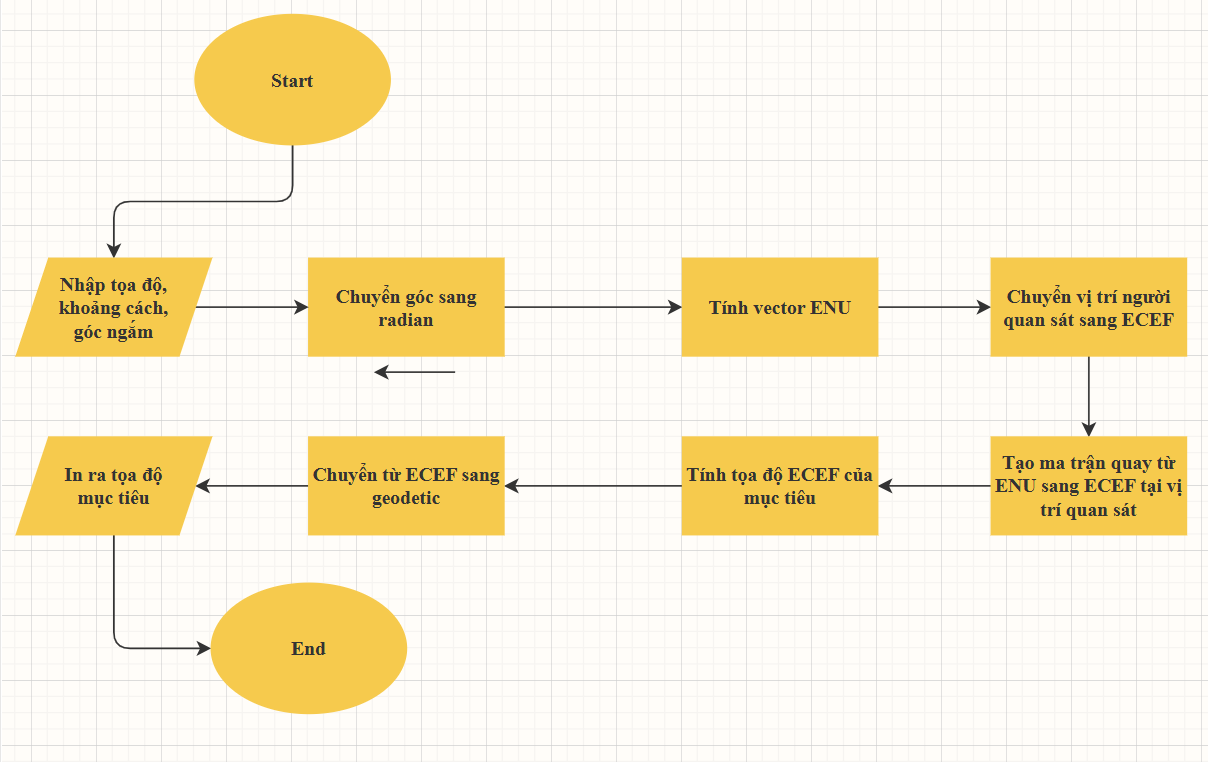
\includegraphics[scale=0.46]{Images/Calc/image.png}
\end{center} 


\item Kết quả tính toán từ Python

\begin{center}
    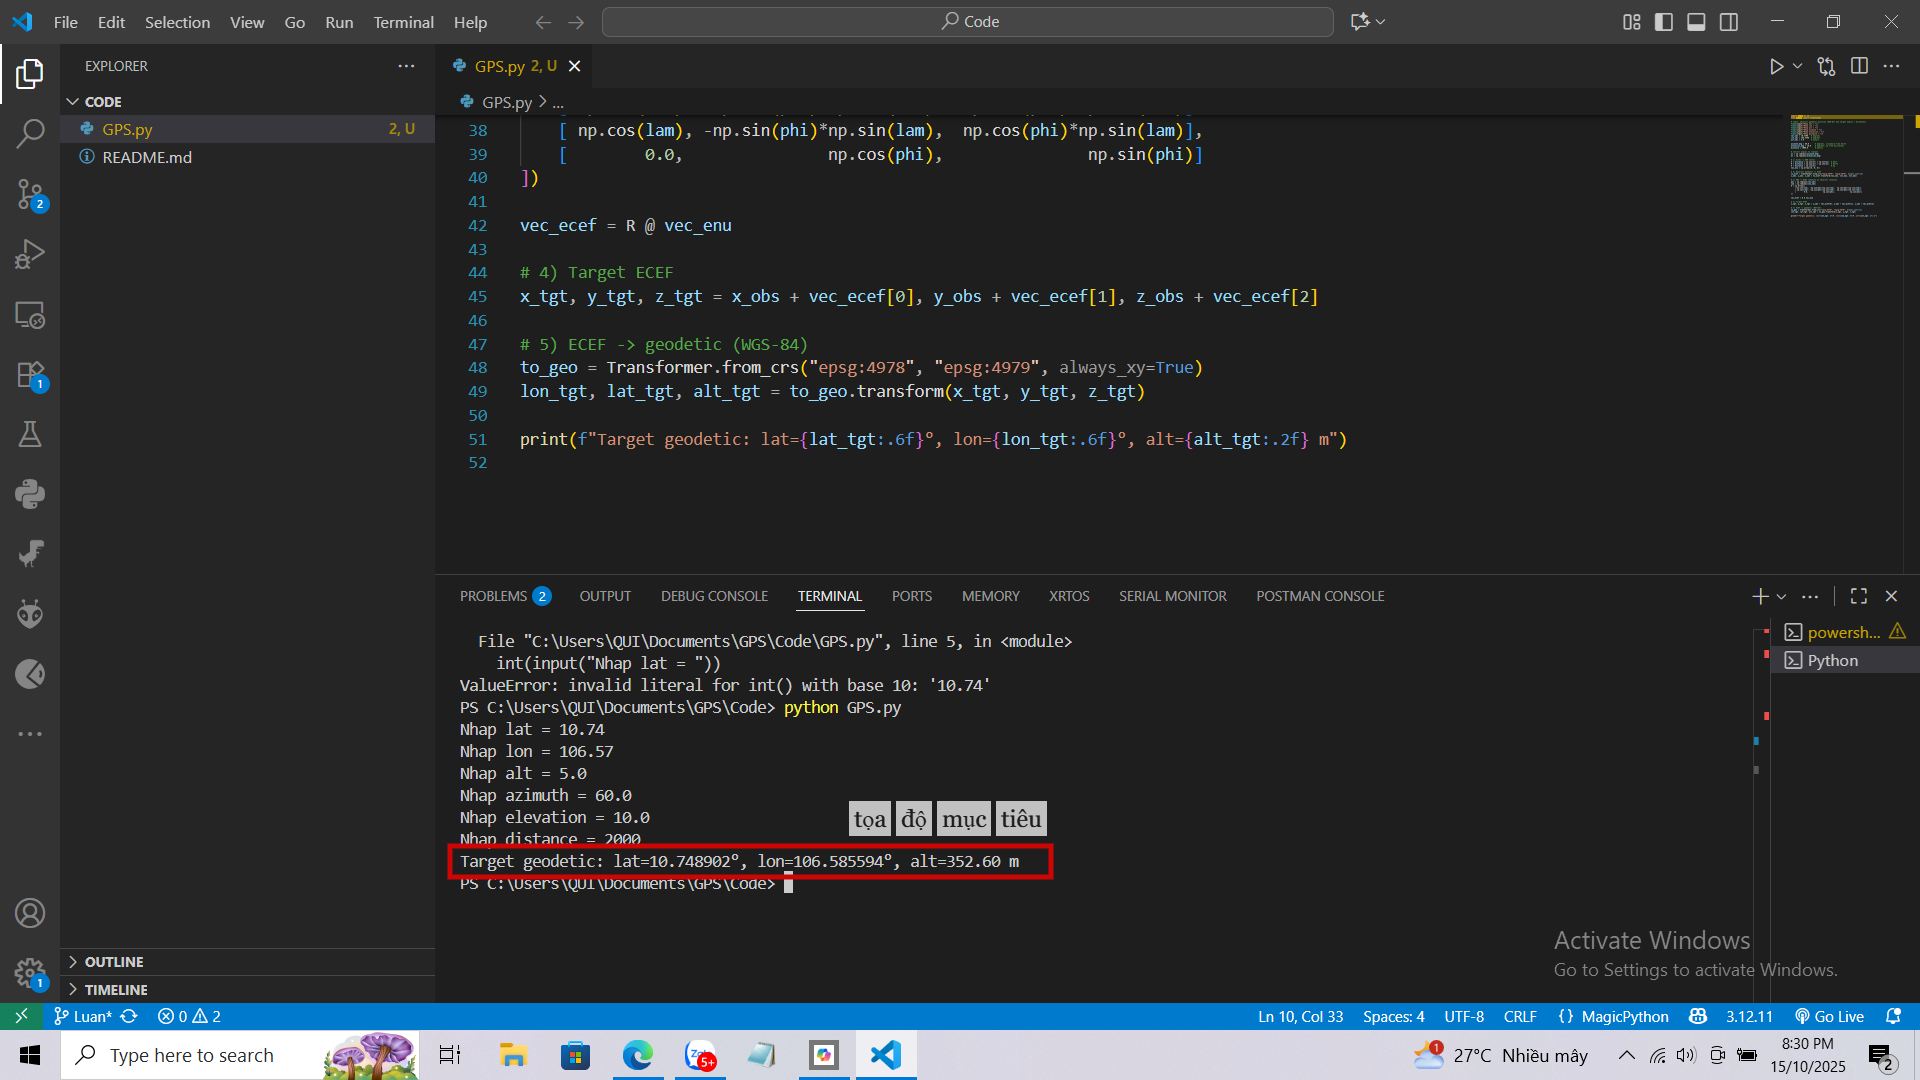
\includegraphics[scale=0.22]{Images/Calc/calcGPS.png}
\end{center}

\newpage
\section{Web Map Use Cases}
\subsection{Tổng quan về Web Map Viewer}
\subsubsection{Định nghĩa về Web Map Viewer}
Web Map Viewer là một ứng dụng hoặc công cụ thực hiện trên nền tảng web cho phép người dùng xem, tương tác và phân tích dữ liệu bản đồ trực tuyến. Trong phạm vi dự án, module này thường được dùng để truy cập các bản đồ và thông tin địa lý, chia sẻ với người khác và tối ưu hóa cho người dùng không chuyên về địa lý.
\subsubsection{Mục tiêu của Web Map Viewer}
\begin{itemize}
    \item Cung cấp giao diện trực quan cho phép xác minh, chia sẻ và xuất tọa độ mục tiêu nhanh chóng (suitable for field operations).
    \item Tích hợp dữ liệu cảm biến (GPS, IMU, laser rangefinder) để chuyển từ đo đạc hướng/khoảng cách sang tọa độ địa lý hiển thị trên bản đồ.
    \item Hỗ trợ đa kịch bản: quân sự, tìm kiếm cứu nạn, trắc địa/GIS, khảo sát xây dựng, quản lý khủng hoảng, nông lâm nghiệp, du lịch, môi trường, hạ tầng, và đào tạo.
    \item Dễ triển khai (static HTML + Leaflet), nhẹ, tương thích trên thiết bị di động và có cơ chế làm việc offline (cached tiles / mbtiles).
\end{itemize}
\subsubsection{Chức năng chính}
Web Map Viewer nên cung cấp một tập hợp chức năng cốt lõi để đáp ứng các use case hiện trường và phân tích sau xử lý:
\begin{itemize}
    \item \textbf{Theo dõi thời gian thực (Real-time Tracking):} hiển thị vị trí observer, team hoặc asset theo timestamp; hỗ trợ streaming vị trí qua WebSocket/HTTP SSE/MQTT.
    \item \textbf{Tích hợp cảm biến (Sensor Integration):} nhận và xử lý trực tiếp dữ liệu GPS, IMU, laser rangefinder (azimuth/elevation/distance), cho phép chuyển đổi hướng + khoảng cách sang tọa độ địa lý và hiển thị trên map.
    \item \textbf{Vẽ, đo đạc và chỉnh sửa không gian (Drawing \& Measurement):} tạo/ sửa marker, polyline, polygon; đo khoảng cách, diện tích; gán thuộc tính metadata cho feature.
    \item \textbf{Quản lý lớp (Layer Management):} bật/tắt layer, điều chỉnh thứ tự hiển thị, thay đổi style/symbol cho từng lớp, hỗ trợ vector và raster tiles.
    \item \textbf{Chuyển đổi hệ toạ độ \& phép chiếu:} hiển thị tọa độ theo nhiều định dạng (DD, DMS), chuyển đổi giữa WGS-84/EPSG:3857/UTM khi cần cho tính toán chính xác.
    \item \textbf{Export/Import dữ liệu:} xuất/nhập GeoJSON, KML, CSV; xuất báo cáo in/PDF và screenshot bản đồ.
    \item \textbf{Offline mode \& caching:} lưu tile/mbtiles cục bộ, lưu tạm các điểm đo, đồng bộ khi có kết nối.
    \item \textbf{Điều hướng và tuyến đường (Routing):} (tuỳ chọn) tính đường đi ngắn nhất, tạo đường dẫn tới điểm đo/target, tích hợp elevation profile cho phân tích địa hình.
    \item \textbf{Alerts, Geofencing \& Notifications:} định nghĩa vùng (geofence) và cảnh báo khi asset vào/ra vùng; gửi cảnh báo tới người dùng/máy chủ.
    \item \textbf{Time slider / Replay:} phát lại lịch sử vị trí theo thời gian để phân tích diễn tiến sự kiện hoặc audit.
    \item \textbf{Bảo mật và phân quyền:} xác thực người dùng, phân quyền theo vai trò, logging hoạt động và chữ ký số cho dữ liệu nhạy cảm.
    \item \textbf{API \& Interoperability:} REST/GraphQL/WebSocket API để tích hợp với hệ thống thứ cấp (backend, command center, database GIS), hỗ trợ xuất dữ liệu cho QGIS/ArcGIS.
\end{itemize}
\subsubsection{Lợi ích khi sử dụng Web Map Viewer}
Sử dụng Web Map Viewer đem lại nhiều lợi ích thiết thực cho các bên liên quan (field operator, analyst, command center, quản lý), cụ thể:
\begin{itemize}
    \item \textbf{Tăng cường nhận thức tình huống (Situational Awareness):} tập hợp và trực quan hoá vị trí, mục tiêu và trạng thái cảm biến giúp người quyết định nắm bắt tình hình nhanh và chính xác hơn.
    \item \textbf{Ra quyết định nhanh hơn và chính xác hơn:} thông tin trực quan, đo đạc tức thời và metadata chất lượng (HDOP, SNR, timestamp) giúp giảm sai sót so với phương pháp thủ công.
    \item \textbf{Hợp tác hiệu quả (Collaboration):} chia sẻ bản đồ/feature/track theo thời gian thực giữa nhiều người dùng, giảm trùng lặp công việc và cải thiện phối hợp tác chiến/ cứu hộ/ khảo sát.
    \item \textbf{Tiết kiệm chi phí và thời gian:} giảm nhu cầu di chuyển lại nhiều lần bằng cách ghi nhận chính xác điểm đo, tái sử dụng dữ liệu; giảm chi phí giấy tờ/hoạt động thủ công.
    \item \textbf{Tính nhất quán và truy vết (Auditability):} lưu lịch sử đo, replay và audit log giúp kiểm chứng thao tác, phục vụ báo cáo hậu kiểm và pháp lý.
    \item \textbf{Khả năng mở rộng và tích hợp:} thiết kế dựa trên chuẩn mở (GeoJSON, REST, EPSG) giúp dễ tích hợp với hệ thống GIS/ERPs khác, mở rộng chức năng khi cần (routing, analytics).
    \item \textbf{Hoạt động trong điều kiện hạn chế kết nối:} chế độ offline và cache cho phép hoạt động trong vùng không có mạng — rất quan trọng cho SAR, công trường, vùng xa.
    \item \textbf{Nâng cao an toàn và tuân thủ:} cơ chế cảnh báo, geofencing và quản lý quyền giúp tuân thủ quy trình an toàn và giảm rủi ro vận hành.
    \item \textbf{Hỗ trợ đào tạo và đánh giá năng lực:} chế độ replay, scoring và record giúp huấn luyện đội ngũ (drills) và đánh giá hiệu năng sau nhiệm vụ.
\end{itemize}
\subsection{Use Cases}
\subsubsection{MILITARY \& DEFENSE}
\textbf{Use case 1.1: Hệ thống kiểm soát hỏa lực pháo binh} \\

\textbf{Scenario:}
\begin{quote}
Một đơn vị pháo binh cần xác định tọa độ mục tiêu để điều chỉnh hỏa lực.
\end{quote}

\textbf{Workflow:}
\begin{enumerate}
    \item \textbf{Observer (Forward Observer)}: Đứng tại vị trí cần quan sát, quan sát mục tiêu
    \item \textbf{Measurement:}
    \begin{itemize}
        \item GPS: Thu thập tọa độ observer
        \item IMU/Compass: Đo góc phương vị đến mục tiêu
        \item Laser Rangefinder: Đo khoảng cách
    \end{itemize}
    \item \textbf{Calculation}: Hệ thống tính tọa độ mục tiêu
    \item \textbf{Visualization}: Hiển thị trên web map
    \item \textbf{Communication}: Chia sẻ liên kết bản đồ HTML với trung tâm kiểm soát hỏa lực
    \item \textbf{Verification}: Verify tọa độ trên map trước khi tiếp cận
\end{enumerate}
\textbf{Web Map Features:}
\begin{itemize}[label=\textbullet]
    \item Cập nhật điểm đánh dấu theo thời gian thực
    \item Hiển thị khoảng cách và phương vị
    \item Hiển thị trực quan đường ngắm
    \item Cửa sổ thông tin tọa độ
    \item Xuất tọa độ cho phần mềm điều khiển hỏa lực
\end{itemize}
\textbf{Benefits:}
\begin{itemize}[label=\textbullet]
    \item \textbf{Accuracy}: Visual verification trước khi bắn
    \item \textbf{Speed}: Chia sẻ tọa độ tức thì
    \item \textbf{Mobility}: Hoạt động trên tablet/phone trong field
    \item \textbf{Offline}: Không cần kết nối Internet
\end{itemize}
\textbf{Screenshot Example:}
\begin{verbatim}
[Observer Marker] ----2.5km----> [Target Marker]
    (Green)                           (Red)


Popup Info:
Observer: 10.762622°, 106.660172°
Target: 10.784523°, 106.683421°
Bearing: 45° (NE)
Distance: 2.5km
Elevation: +15° (target above observer)
\end{verbatim}
\textbf{Use case 1.2: Chỉ định mục tiêu UAV/Drone} \\

\textbf{Scenario:}
\begin{quote}
UAV operator cần designate target cho surveillance hoặc strike mission.
\end{quote}

\textbf{Workflow:}
\begin{enumerate}
    \item Người điều khiển UAV xác định mục tiêu trực quan
    \item Ghi lại vị trí GPS + góc gimbal
    \item Tính toán tọa độ mục tiêu
    \item Hiển thị trên bản đồ web với đường bay
    \item Chia sẻ bản đồ với trung tâm chỉ huy
    \item Cập nhật trạng thái mục tiêu theo thời gian thực
\end{enumerate}
\textbf{Web Map Features:}
\begin{itemize}[label=\textbullet]
    \item Nhiều mục tiêu trên một bản đồ
    \item Đánh dấu mã màu (mức độ đe dọa)
    \item Lớp phủ đường bay
    \item Cập nhật vị trí theo thời gian thực
    \item Chỉ báo mức độ ưu tiên của mục tiêu
\end{itemize}
\textbf{Benefits:}
\begin{itemize}[label=\textbullet]
    \item \textbf{Situational Awareness}: Xem tất cả mục tiêu trên một bản đồ
    \item \textbf{Real-time Updates}: Theo dõi mục tiêu động
    \item \textbf{Precision}: Xác minh tọa độ trước khi giao chiếnt
\end{itemize}
\subsubsection{Search \& Rescue (SAR)}
\textbf{Use case 2.1: Vị trí người mất tích} \\

\textbf{Scenario:}
\begin{quote}
Đội SAR cần xác định vị trí người mất tích trong rừng/núi.
\end{quote}

\textbf{Workflow:}
\begin{enumerate}
    \item \textbf{Initial Report}: Nhận tọa độ vị trí cuối cùng được biết đến
    \item \textbf{Search Pattern}: Chia khu vực thành các sectors
    \item \textbf{Team Deployment}: Mỗi đội báo cáo vị trí + tìm kiếm
    \item \textbf{Target Spotted}: Đội báo cáo azimuth/distance đến subject
    \item \textbf{Coordinate Calculation}: Tính toán vị trí chính xác
    \item \textbf{Web Map Update}: Đánh dấu vị trí, chia sẻ với tất cả teams
    \item \textbf{Rescue Coordination}: Điều dẫn đội ngũ y tế đến địa điểm chính xác
\end{enumerate}
\textbf{Web Map Features:}
\begin{itemize}[label=\textbullet]
    \item Đánh dấu nhiều đội (nhiều màu khác nhau)
    \item Lớp phủ khu vực tìm kiếm
    \item Vòng tròn khoảng cách (bán kính tìm kiếm)
    \item Tùy chọn bản đồ địa hình
    \item Đánh dấu vị trí cuối cùng được biết đến
\end{itemize}
\textbf{Benefits:}
\begin{itemize}[label=\textbullet]
    \item \textbf{Time Critical}: Nhanh chóng phối hợp các nỗ lực cứu hộ
    \item \textbf{Precision}: Vị trí chính xác để sơ tán y tế
    \item \textbf{Coordination}: Tất cả các đội đều nhìn thấy cùng một bản đồ
    \item \textbf{Offline Maps}: Làm việc trong vùng không có vùng phủ sóng di động
\end{itemize}
\textbf{Use case 2.2: Maritime Search \& Rescue} \\

\textbf{Scenario:}
\begin{quote}
Coast guard tìm kiếm tàu gặp nạn trên biển.
\end{quote}

\textbf{Workflow:}
\begin{enumerate}
    \item Tín hiệu cấp cứu được nhận với tọa độ gần đúng
    \item Tàu/máy bay được triển khai đến khu vực tìm kiếm
    \item Quan sát bằng mắt thường: Ghi lại hướng/khoảng cách từ tàu
    \item Tính toán tọa độ hiệu chỉnh độ trôi
    \item Bản đồ web hiển thị:
    \begin{itemize}
        \item vị trí tàu tìm kiếm
        \item vị trí cuối cùng được biết của mục tiêu
        \item vị trí hiện tại
        \item Đường đi dự đoán trôi dạt
    \end{itemize}
    \item Phối hợp các hoạt động cứu hộ
\end{enumerate}
\textbf{Web Map Features:}
\begin{itemize}[label=\textbullet]
    \item Tỷ lệ hải lý
    \item Lớp phủ dòng chảy/gió (nếu có)
    \item Hình ảnh hóa mẫu tìm kiếm
    \item Đánh dấu vị trí có dấu thời gian
\end{itemize}
\subsubsection{Tourism \& Recreation}
\textbf{Use case 3.1: Điều hướng đường mòn} \\

\textbf{Scenario:}
\begin{quote}
Người đi bộ sử dụng hệ thống để điều hướng và đánh dấu các điểm ưa thích.
\end{quote}

\textbf{Workflow:}
\begin{enumerate}
    \item Bắt đầu đi bộ đường dài: ghi lại GPS điểm đầu đường mòn
    \item Đánh dấu các điểm dừng dọc đường mòn
    \item Ghi chú các điểm thú vị (điểm ngắm cảnh, khu cắm trại)
    \item Tính toán khoảng cách giữa các điểm
    \item Chia sẻ bản đồ đường mòn với những người đi bộ đường dài khác
    \item Tải lên cơ sở dữ liệu đường mòn
\end{enumerate}
\textbf{Web Map Features:}
\begin{itemize}[label=\textbullet]
    \item Lớp phủ đường mòn
    \item Độ cao (nếu có)
    \item Điểm đánh dấu ảnh
    \item Tạo liên kết chia sẻ
\end{itemize}
\subsubsection{Education \& Training}
\textbf{Use case 4.1: Bài tập huấn luyện quân sự} \\

\textbf{Scenario:}
\begin{quote}
Huấn luyện quân đội về quy trình chỉ định mục tiêu.
\end{quote}

\textbf{Workflow:}
\begin{enumerate}
    \item Giảng viên thiết lập kịch bản đào tạo
    \item Học viên thực hành đo mục tiêu
    \item Gửi tọa độ qua giao diện web
    \item Hệ thống tính toán độ chính xác
    \item Bản đồ web hiển thị tất cả bài nộp của học viên so với thực tế
    \item Tóm tắt với phân tích trực quan
\end{enumerate}
\textbf{Web Map Features:}
\begin{itemize}[label=\textbullet]
    \item Nhiều người dùng gửi bài
    \item Hiển thị lỗi (khoảng cách so với thực tế)
    \item Hệ thống chấm điểm
    \item Khả năng phát lại
\end{itemize}
\subsection{Technical Architecture}
\subsubsection{System Components}

\begin{center}
    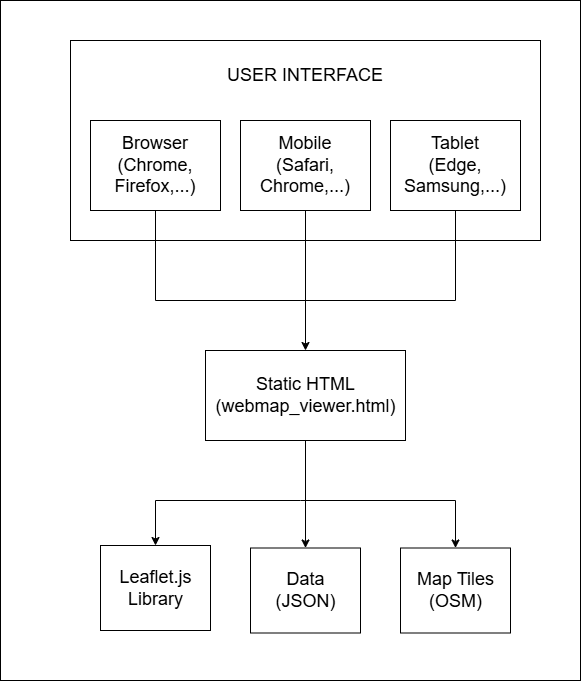
\includegraphics[scale=0.5]{Images/webmap_system_components.png}
\end{center}

\subsubsection{Technology Stack}
\paragraph{Frontend}
\begin{itemize}[label=\textbullet]
    \item \textbf{HTML5}: Structure \& semantics
    \item \textbf{CSS3}: Styling \& responsive design
    \item \textbf{JavaScript ES6}: Logic \& interactivity
    \item \textbf{Leaflet.js 1.9.4}: Mapping engine
\end{itemize}
\paragraph{Data Formats}
\begin{itemize}[label=\textbullet]
    \item \textbf{GeoJSON}: Geographic data exchange
    \item \textbf{JSON}: Configuration \& metadata
    \item \textbf{CSV}: Bulk data import/export
\end{itemize}
\paragraph{Map Services}
\begin{itemize}[label=\textbullet]
    \item \textbf{OpenStreetMap}: Base map tiles
    \item \textbf{Alternatives}: Stamen Terrain, CartoDB, Mapbox
\end{itemize}
\end{itemize}

\newpage
\subsection{Prototype phần mềm mô phỏng (Leaflet Web Map)}
\textbf{Trang web triển khai:} \href{https://kzeyrox45.github.io/GPS-Target-Calculating-System/}{kzeyrox45.github.io/GPS-Target-Calculating-System}
\subsubsection{Mục tiêu}
Phần mềm mô phỏng được xây dựng nhằm trực quan hoá kết quả tính toán toạ độ mục tiêu từ dữ liệu đo (toạ độ người quan sát, góc ngắm và khoảng cách). 
Giao diện cho phép người dùng nhập thông tin đầu vào, tính toán toạ độ mục tiêu và hiển thị kết quả ngay trên bản đồ thực tế, giúp dễ dàng kiểm chứng tính chính xác của mô hình.

\subsubsection{Công nghệ sử dụng}
\begin{itemize}
    \item \textbf{HTML, CSS, JavaScript:} Xây dựng giao diện người dùng và xử lý sự kiện nhập liệu.
    \item \textbf{Leaflet.js:} Thư viện bản đồ mã nguồn mở, hiển thị bản đồ nền (OpenStreetMap) và các marker.
    \item \textbf{OpenStreetMap (OSM):} Nguồn dữ liệu bản đồ miễn phí được Leaflet sử dụng.
\end{itemize}

\subsubsection{Cấu trúc giao diện}
Giao diện chính của hệ thống được chia thành hai phần:
\begin{enumerate}
    \item \textbf{Khung nhập dữ liệu:} Bao gồm các trường nhập
    \begin{itemize}
        \item Toạ độ người quan sát (vĩ độ, kinh độ).
        \item Góc ngắm (đơn vị độ, tính từ hướng Bắc).
        \item Khoảng cách tới mục tiêu (đơn vị km).
    \end{itemize}
    \item \textbf{Bản đồ hiển thị:} Hiển thị vị trí người quan sát, mục tiêu và hướng ngắm.
\end{enumerate}

\noindent
Các phần tử trên bản đồ gồm:
\begin{itemize}
    \item Marker màu đỏ : vị trí người quan sát.
    \item Marker màu xanh : vị trí mục tiêu được tính toán.
    \item Đường đứt nét (--): biểu diễn hướng ngắm.
    \item Khung chú giải: hiển thị ý nghĩa các ký hiệu.
\end{itemize}


\begin{figure}[H]
    \centering
    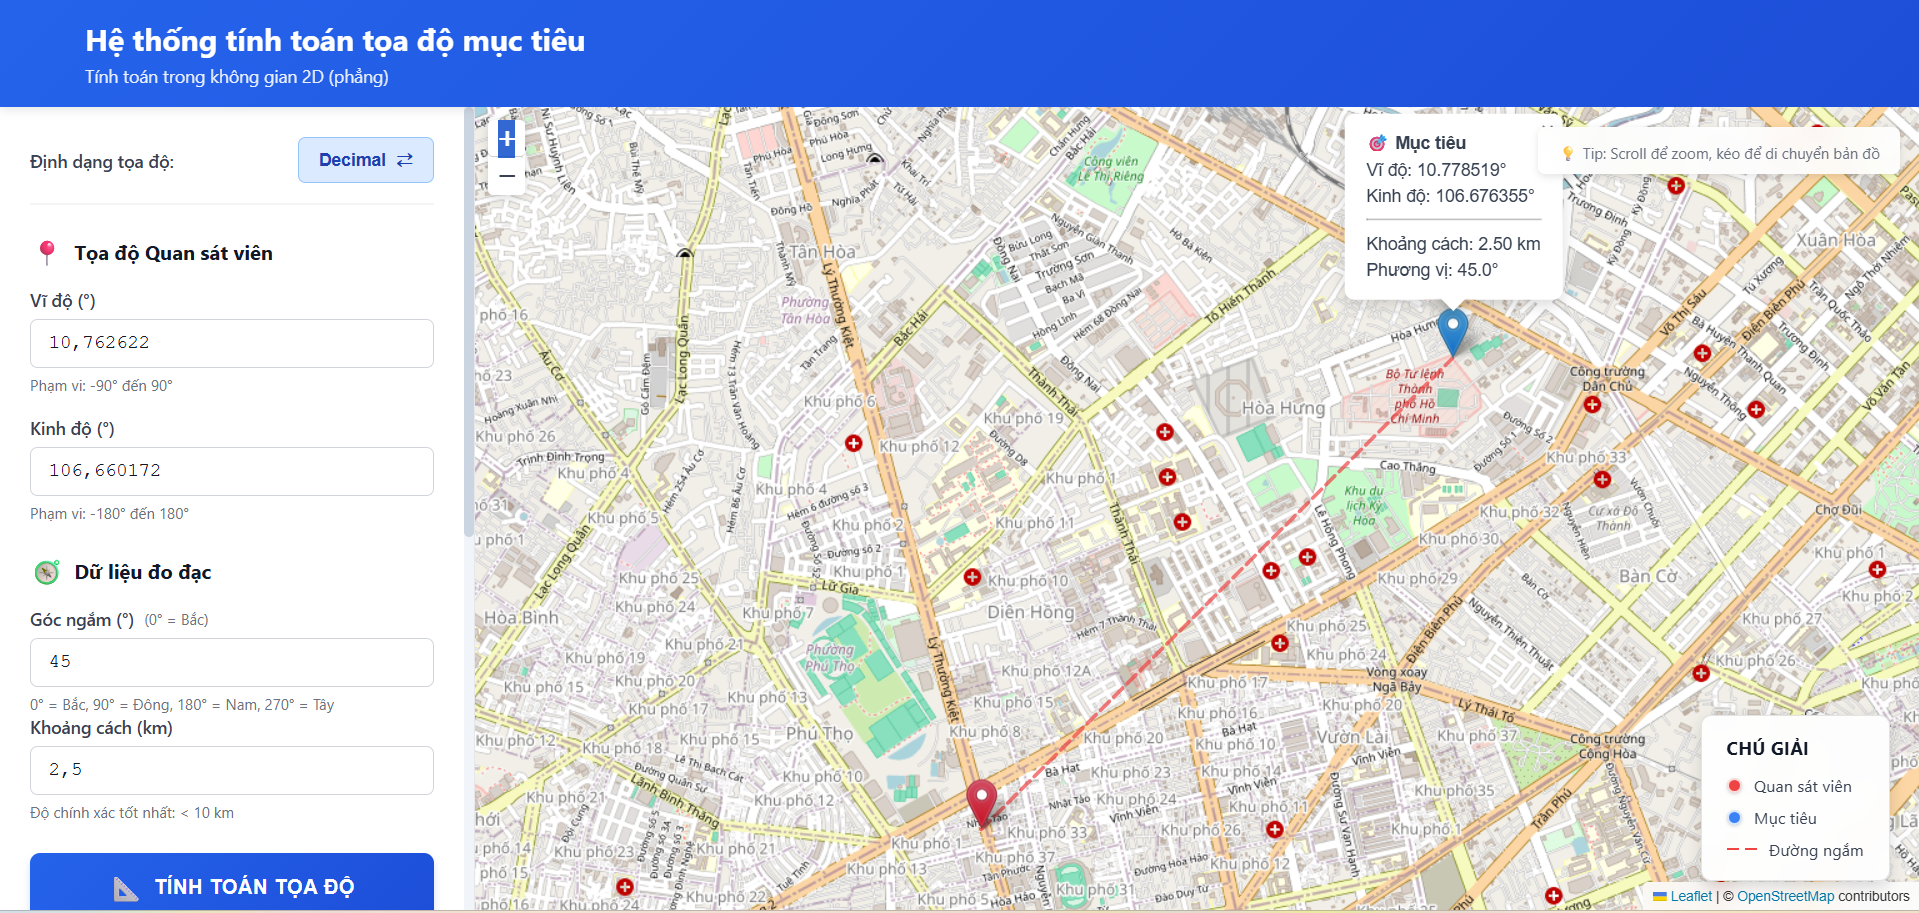
\includegraphics[scale=0.3]
    {Images/webmap_interface.png}
    \vspace{0.8cm} 
    \caption{Giao diện hệ thống tính toán toạ độ mục tiêu trên bản đồ Leaflet}
\end{figure}

\newpage

Hệ thống cho phép người dùng lựa chọn định dạng nhập tọa độ ở hai dạng phổ biến là \textbf{Decimal} (độ thập phân) và \textbf{DMS} (Degrees–Minutes–Seconds, tức độ–phút–giây). 
Người dùng có thể chuyển đổi linh hoạt giữa hai định dạng thông qua nút “\textit{Định dạng tọa độ: DMS và Decimal}”, giúp thuận tiện trong việc nhập liệu theo các nguồn dữ liệu đo đạc khác nhau.

\begin{figure}[H]
    \centering
    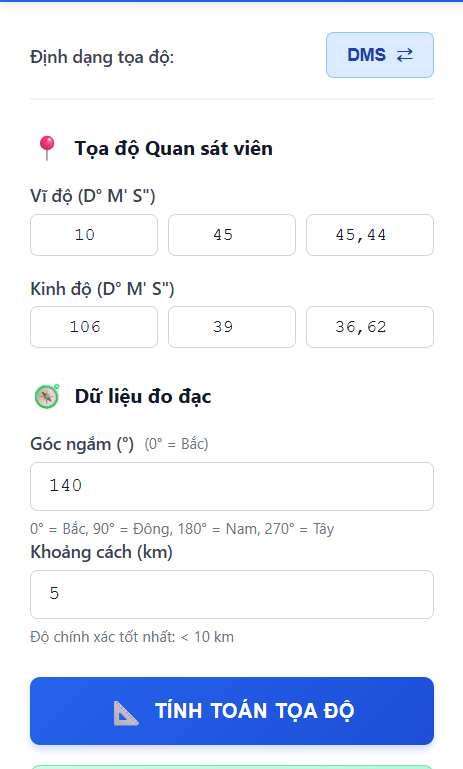
\includegraphics[scale=0.33]
    {Images/webmap_interface_dms.png}
    \vspace{0.8cm} 
    \caption{Giao diện hệ thống tính toán toạ độ mục tiêu trên bản đồ Leaflet}
\end{figure}

\subsubsection{Nguyên lý hoạt động}
Khi người dùng nhập các thông số đầu vào, hệ thống sẽ:
\begin{enumerate}
    \item Lấy dữ liệu toạ độ người quan sát $(lat_1, lon_1)$, góc ngắm $\theta$ và khoảng cách $d$.
    \item Thực hiện phép tính toạ độ mục tiêu theo mô hình toạ độ cực.
    \item Hiển thị vị trí người quan sát và mục tiêu trên bản đồ OpenStreetMap thông qua Leaflet và bảng dữ liệu chi tiết.
\end{enumerate}

\subsubsection{Kết quả mô phỏng}
Sau khi nhập dữ liệu và nhấn nút \textit{“Tính toán toạ độ”}, hệ thống hiển thị kết quả trực tiếp trên bản đồ:
\begin{itemize}
    \item Toạ độ mục tiêu được hiển thị bằng marker màu xanh.
    \item Hướng ngắm được thể hiện bằng đoạn thẳng nối hai vị trí.
    \item Thông tin chi tiết của từng điểm được hiển thị khi người dùng rê chuột vào marker, hoặc kéo xuống và xem bảng "Tọa độ Mục tiêu"
\end{itemize}

\begin{figure}[H]
    \centering
    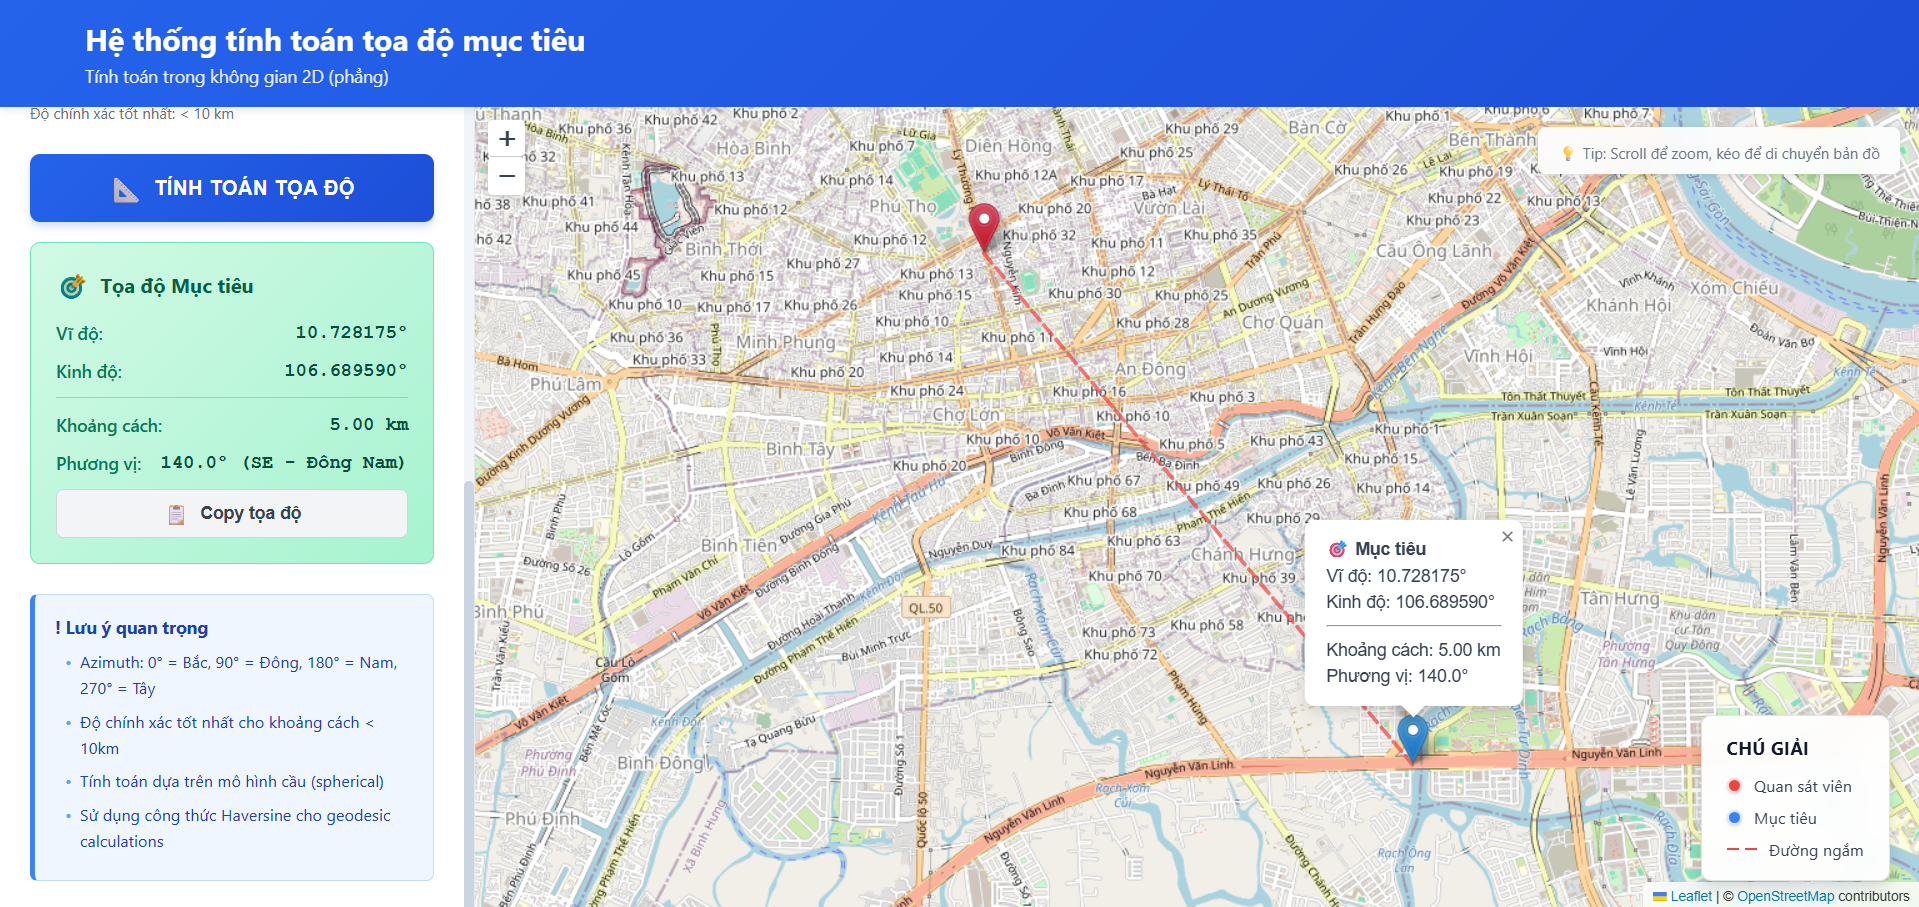
\includegraphics[scale=0.33]
    {Images/webmap_result.png}
    \vspace{0.8cm} 
    \caption{Giao diện hệ thống tính toán toạ độ mục tiêu trên bản đồ Leaflet}
\end{figure}

\subsubsection{Đánh giá}
Prototype phần mềm mô phỏng đã đáp ứng yêu cầu trực quan hoá kết quả tính toán, giúp người dùng dễ dàng xác định vị trí mục tiêu trong không gian phẳng 2D. 
Hệ thống có thể mở rộng để làm việc với bản đồ 3D hoặc kết nối với cơ sở dữ liệu cảm biến thực tế trong các nghiên cứu tiếp theo.
